\chapter{Einleitung}
\label{chap:einleitung}
    Um den Abschluss des Fachhochschul-Bachelorstudiengangs Software Engineering an
    der FH Hagenberg zu erlangen, muss im Rahmen des Studiums ein zwölfwöchiges Berufspraktikum absolviert werden. Dieses Praktikum wird in der Regel im sechsten
     Semester absolviert und erfordert die Zusammenarbeit mit einem von der FH geprüften
    Unternehmen oder einer Einrichtung. Anschließend ist dazu ein Bericht abzugeben, der
    die Tätigkeiten und Ergebnisse des Praktikums beschreibt.

\section{Unternehmen und Arbeitsumfeld}\label{sec:unternehmen-und-arbeitsumfeld}
    Das Praktikum wurde bei \emph{ITPRO - Consulting \& Software GmbH} \cite{ITPRO} absolviert. Dabei handelt es sich um ein Unternehmen, das sich auf die Entwicklung von Softwarelösungen 
    spezialisiert hat. Gegründet wurde es im Jahre 1999 und hat seinen Hauptsitz in Linz. Kleinere Büros befinden sich in Hagenberg und Ottensheim. Derzeit sind insgesamt um die 
    50 Mitarbeiter*innen in den verschiedenen Büros beschäftigt. Diese können bis auf wenige Ausnahmen frei zwischen den Büros wechseln und dort arbeiten. 
    
    Unter normalen Umständen sind um die 8 Mitarbeiter*innen  aus 2 verschiedenen Teams im Hagenberger Standort anzutreffen.
    Der Großteil des Praktikums wurde aus diesem Grund in Hagenberg absolviert.
    ITPRO bietet Außendienst-Lösungen, Dienstleistungs-ERP, Lösungen für \gls{oepnv}-Unter-nehmen und individuelle Software-Lösungen an, für die auch individuelle Hardware entwickelt
    und ausgeliefert wird.

    Das Praktikum sah eine Stelle als Entwickler im internen Team \emph{"Team Nachtschicht"} vor. Der Name wurde von den Entwicklern gewählt und ihm kann keinerlei tiefere Bedeutung zugeordnet werden.
    Dieses Team besteht derzeit aus 11 Personen und ist für die Entwicklung 
    von \gls{oepnv}-Lösungen zuständig. Als Vorgehensmodell des Projektmanagements wird Scrum verwendet. Die Technologien werden auf Absprache mit dem Kunden ausgewählt. Gibt es von deren Seite keine
    Präferenz, so wird in der Regel auf C\# und .NET zurückgegriffen.

    Obwohl die Teilnahme an Scrum-Meetings verpflichtend war, wurde mit nur wenigen Ausnahmen, ausschließlich mit 2 Mitarbeitern zusammengearbeitet. Dabei handelte es sich einerseits um Herrn Julian Gaisbauer 
    BSc, der die Rolle des Betreuers im Praktikum übernommen hat. Dieser war mit der Einarbeitung in die Projekte und der Unterstützung bei der Arbeit betraut. Außerdem stand er für 
    Fragen und Probleme aller Art zur Verfügung. Die zweite Person war Herr Theodor Hartleitner MSc, der einen Großteil der Aufgaben und Anforderungen definierte. Bei spezifischeren 
    Fragen zu den Anforderungen und der Software stand er ebenfalls zur Verfügung. Mit den anderen Teammitgliedern wurde wenig Zusammenarbeit geleistet, da diese meist an anderen Projekten arbeiteten.


\section{Übersicht über die Projekte}\label{sec:ueberblick-projekte}
    Während der Zeit des Praktikums wurde an zwei Projekten gearbeitet. Beide Projekte sind im Bereich des \gls{oepnv} angesiedelt und sollten somit Verkehrsunternehmen die Verwaltung von ihren Daten 
    vereinfachen. Das Projekt \emph{"ITCS-Management"} sollte dabei die Visualisierung und Verwaltung von Daten wie Fahrpläne und Fahrzeuge ermöglichen. Das zweite Projekt 
    \emph{"ITCS"} sollte eine Schnittstelle zu anderen Systemen bieten, sodass Daten aus anderen Systemen importiert und exportiert werden können. Weiters fungierte es als Bibliothek, 
    die von anderen Projekten verwendet werden kann, um beispielsweise Datenvalidierung zu ermöglichen oder Datenbankobjekte automatisch zu generieren. Die Abkürzung \emph{"ITCS"} steht dabei für
    \emph{"Intermodal Transport Control System"}, was ein Rechnerverbund-System im \gls{oepnv} beschreibt, das Betriebsdaten auf einem zentralen Server sammelt und den Planungsdaten gegenüberstellt \cite{itcs}.
    
\subsection{Das Projekt \emph{"ITCS-Management"}}\label{sec:itcs-management}
    Das Projekt \emph{"ITCS-Management"} ist eine Webanwendung, die es ermöglicht, Daten wie Fahrpläne, Fahrzeuge und Haltestellen zu verwalten. Es wurde mit dem Ziel entwickelt, den 
    Verwaltungsaufwand für Verkehrsunternehmen zu reduzieren und eine benutzerfreundliche Oberfläche zu bieten. Es wurde mit C\# und Blazor umgesetzt. 
    
    Bei der Datenbank
    handelt es sich um eine SQL-Server-Datenbank, die ein VDV-452~\cite{VDV452} konformes
    Datenmodell österreichischer Verkehrsunternehmen abbildet. Gelegentlich musste dieses
    Schema auch erweitert oder angepasst werden. Der Zugriff auf die Datenbank erfolgte durch das \gls{efc}. 
    Das Projekt wurde nicht neu begonnen, sondern  um neue Seiten und Funktionen erweitert.
    Die aufwändigste Aufgabe war dabei die Implementierung der Seite "Umlaufeditor", die die Erstellung und Verwaltung von Umläufen ermöglicht. 
    Umläufe sind eine Zusammenstellung von Fahrten, die von einem Fahrzeug an einem Tag durchgeführt werden.
    % \begin{figure}[H]
    %     \centering
    %     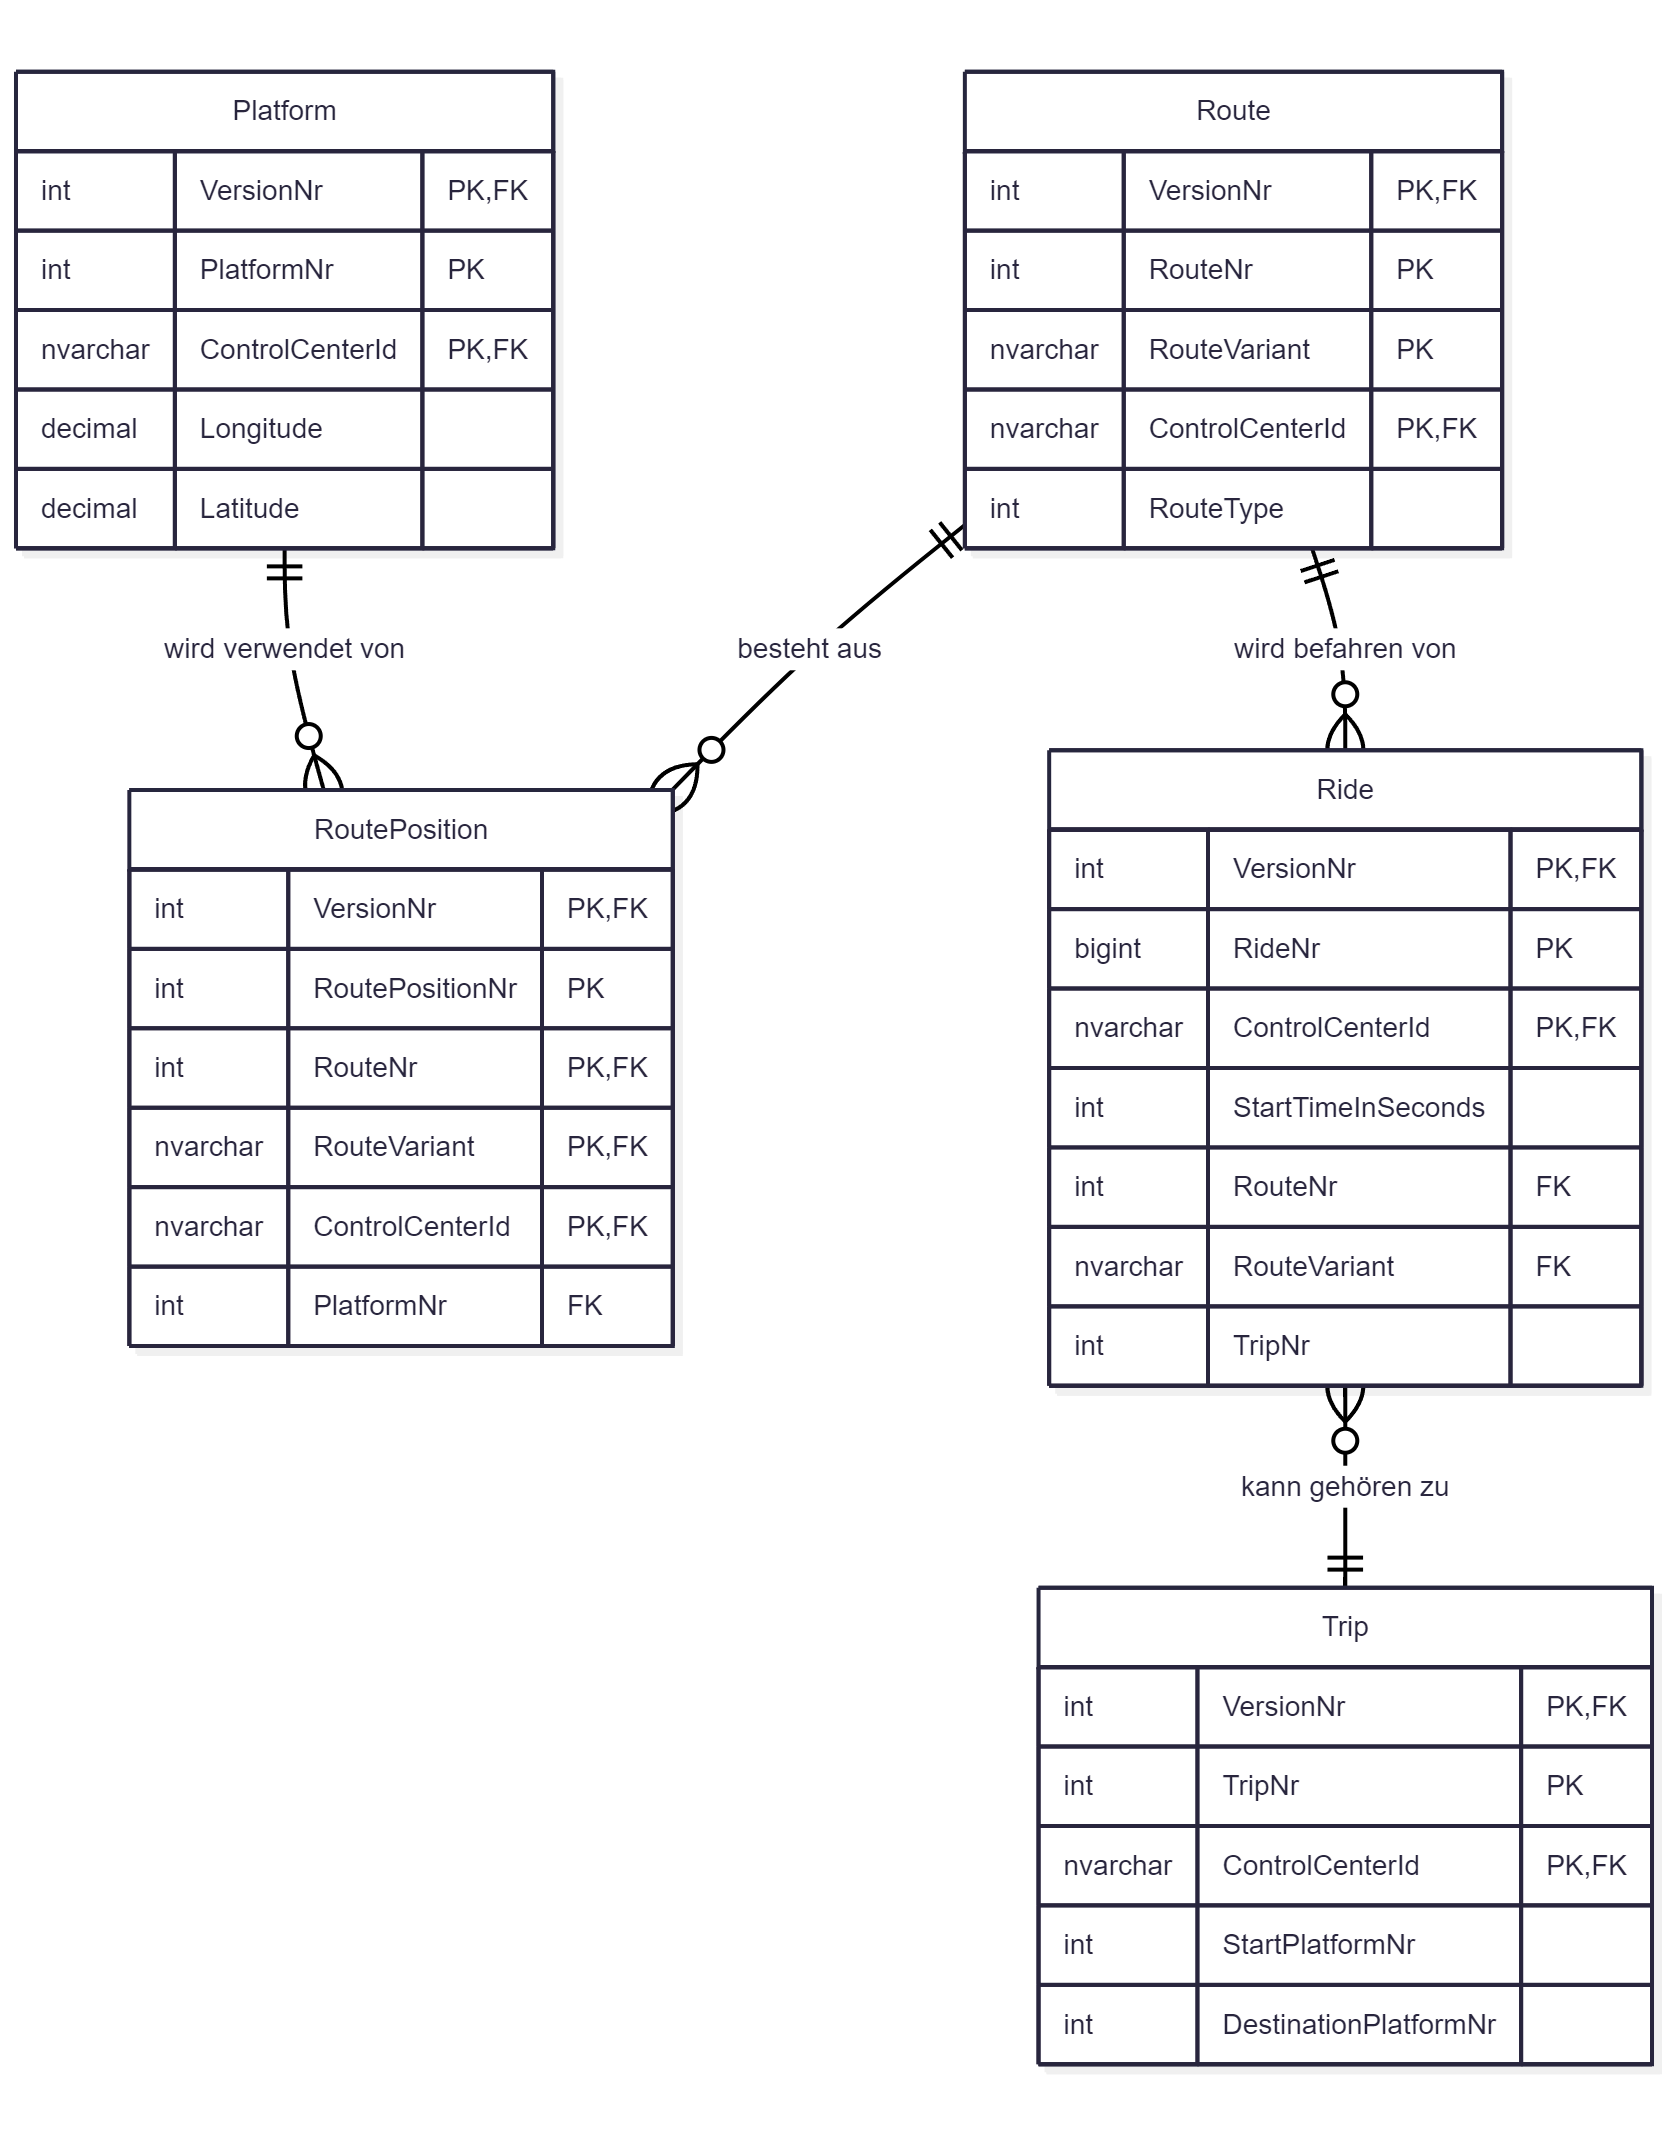
\includegraphics[width=0.95\textwidth]{ER1.png}
    %     \caption{ER-Diagramm eines Ausschnitts des VDV-452 Datenmodells}
    %     \label{fig:VTs}
    % \end{figure}
    Diese Seite ermöglicht es, Umläufe zu erstellen, zu bearbeiten und zu löschen. Diese Umläufe werden in Echtzeit validiert um zeitliche oder räumliche Konflikte zu vermeiden. Bei 
    Bedarf können auch Objekte wie Leerfahrten automatisch erstellt werden.

\subsection{Das Projekt \emph{"ITCS"}}\label{sec:itcs}
    Das zweite Projekt, an dem im Praktikum gearbeitet wurde, ist das Projekt \emph{"ITCS"}. Dieses Projekt stellt eine Ansammlung von Bibliotheken dar.
    Es wurde ebenfalls mit C\# und .NET umgesetzt und bietet verschiedene Schnittstellen zu anderen Systemen wie \emph{sFGM}~\cite{sFGM}.
    Beispiele dafür sind Import- und Exportroutinen, die es ermöglichen, Daten aus anderen Systemen zu importieren und zu exportieren. Diese laufen in der Regel als Hintergrund-Service und gleichen die Daten in
    bestimmten Intervallen ab. Aufgabe im Praktikum war es, die automatische 
    Importierung der auf der ITCS-Datenbank neu erstellten Tabellen zu ermöglichen. Beim Export sollten diese Daten, leicht aufbereitet, in ein System, das für die Verwaltung von 
    Anzeigetafeln verwendet wird, übertragen werden können. Außerdem stellen diese Bibliotheken noch andere Schnittstellen zur Verfügung, die eine automatische Generierung
    von Datenbankobjekten oder Strecken- und Zeitberechnungen ermöglichen. Diese Teile wurden auch im Projekt \emph{"ITCS-Management"} verwendet.
    \begin{figure}[H]
        \centering
        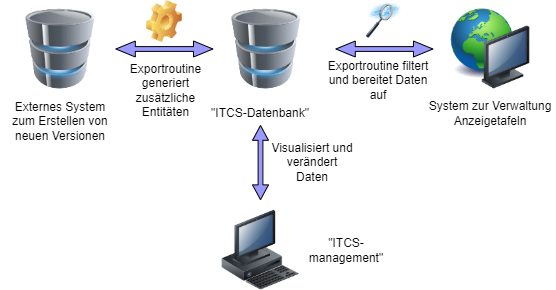
\includegraphics[width=0.9\textwidth]{overview_alt.png}
        \caption{Übersicht über die Projekte}
        \label{fig:VTs}
    \end{figure}

\subsection{Aufgabenstellungen des Praktikanten}\label{sec:aufgabenstellung-praktikant}

    Das Praktikum wurde nicht, wie oft üblich, als eigenes Projekt durchgeführt, sondern als
    Unterstützung für andere größere Projekte, an denen das Team schon länger arbeitete. Somit wurden die Aufgabenstellungen in Form von Tasks vom Product Owner und dem Betreuer definiert 
    und dem Praktikanten zugewiesen. Diese Aufgaben waren auch anfangs nicht vollständig festgelegt, sondern wurden erst bei Bedarf im Detail definiert. Dadurch waren dem Praktikanten zu Beginn
    nur die unmittelbaren Aufgaben bekannt, die in den Meetings mit dem Product Owner besprochen wurden.
    
    Die ersten Aufgaben wiesen nur wenige Zusammenhänge untereinander auf, da diese meist nur wenig Aufwand darstellten und nur wenige Stunden in Anspruch nahmen. 
    Kontakt mit Kunden oder anderen Personen außerhalb des Unternehmens waren nicht Teil des Praktikums und auch die Teilnahme an Team-Meeting war bis auf die Daily-Meetings nicht vorgesehen.
    
    Die wohl umfangreichste Aufgabe war die Implementierung des  \emph{"Umlaufeditors"} im Projekt \emph{"ITCS-Management"} der aus drei verschiedenen Blazor-Seiten besteht. Eine sollte die Erstellung 
    und Verwaltung von Sonderhaltestellen und Betriebshöfen ermöglichen, die zweite die Zusammenstellung von Umläufen, welche eine Zusammenstellung von Fahrten darstellen, und 
    die dritte die Verwaltung von Vorlagen für Umläufe. Diese Vorlagen sollten es später ermöglichen, beim Import neuer Versionen, Umläufe automatisch zu generieren. Im Hintergrund sollte dabei
    die Durchführbarkeit der Umläufe überprüft werden, sodass Konflikte wie zeitliche Überschneidungen oder räumliche Konflikte vermieden werden können. 
    
    Zusätzlich musste dem 
    Endkunden die Möglichkeit gegeben werden, Leerfahrten und Pausen automatisch zu generieren, um die Umläufe zu vervollständigen und räumliche Konflikte zu vermeiden. Die Zuordnung 
    von Fahrten zu Umläufen sollte über Drag \& Drop möglich sein und die Validierung sollte, wenn möglich, in Echtzeit erfolgen. Um dies zu ermöglichen, muss bei der Erstellung von Leerfahrten die 
    zurückzulegende Strecke und Fahrtdauer ebenfalls in Echtzeit ermittelt werden.
    
    Das Konzept des visuellen Designs wurde als Anhaltspunkt über die Design-Plattform "Figma"~\cite{figma} bereitgestellt. Dieses wurde in Absprache mit dem Betreuer und dem 
    Product Owner im Laufe der Entwicklung
    angepasst und erweitert. Die Implementierung der Seiten musste mit "Blazor"~\cite{blazor}, einem Web-UI-Framework von Microsoft, das es ermöglicht, interaktive Webanwendungen mit C\# zu erstellen, erfolgen.
    
    \begin{figure}[H]
        \centering
        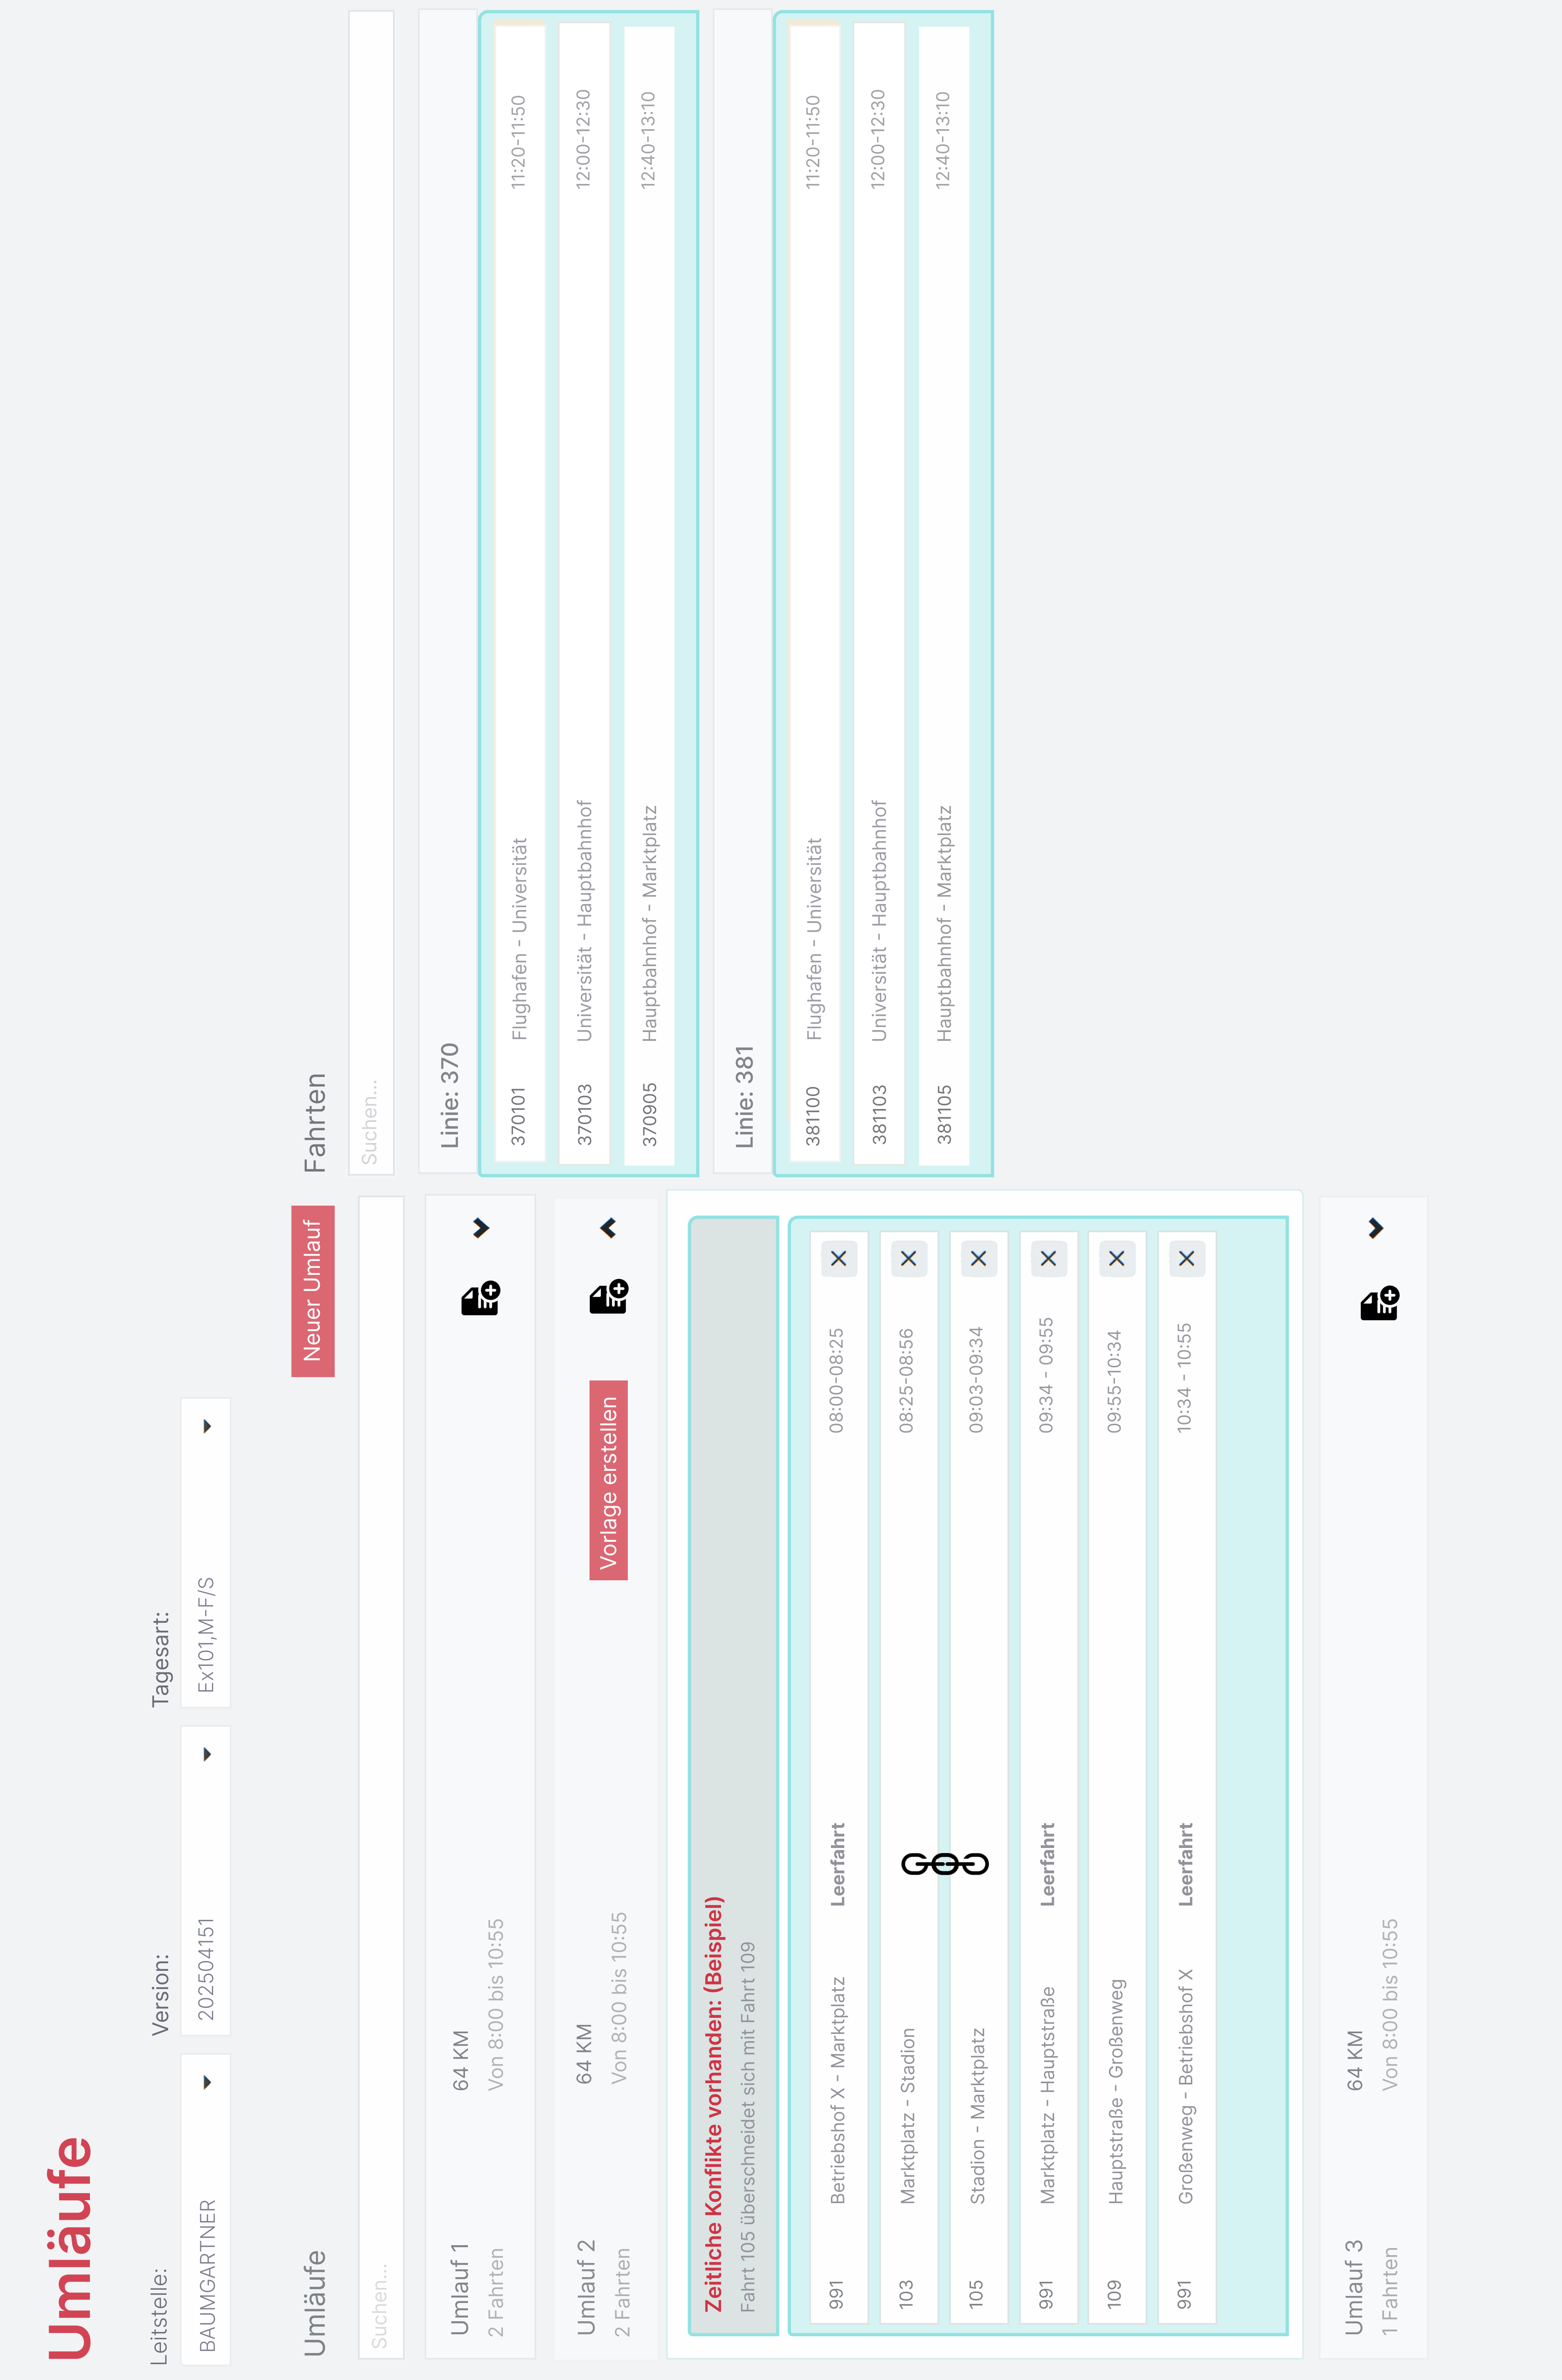
\includegraphics[width=0.95\textwidth]{Umlaufeditor_konzept.png}
        \caption{Erstes Konzept des Umlaufeditors in Figma}
        \label{fig:Umlaufeditor_konzept}
    \end{figure}

    In Abbildung~\ref{fig:Umlaufeditor_konzept} ist das erste Konzept des Umlaufeditors zu sehen. Dabei sollten einzelne Fahrten mit der Maus von der rechten Seite in die Umläufe auf der linken Seite
    gezogen werden können. Die Kettensymbole markieren Anschlussfahrten. Diese erzwingen es, dass die eine Fahrt direkt in die nächste übergeht. Sollte eine solche 
    Fahrt einem Umlauf zugeordnet werden, so wird die gesamte Kette in den Umlauf übernommen.
